\documentclass{article}
\usepackage{graphicx} % Required for inserting images
\usepackage{amsmath}
\usepackage{amssymb}
\usepackage{graphicx}
\usepackage{geometry}
\geometry{margin=1in}
\usepackage[table,xcdraw]{xcolor}

\title{Fpa}
\author{sharmin mim}
\date{November 2024}

\begin{document}

\section*{3. Description and Circuit Diagram of Modules}

To ensure modularity in the design of the floating-point adder, several specialized libraries have been developed and implemented. Below are the descriptions and uses of these libraries.

\subsection*{Input Splitter}
This module splits a 32-bit floating-point number into three parts:
\begin{itemize}
    \item \textbf{1-bit sign}: Determines the sign of the number (positive or negative).
    \item \textbf{11-bit exponent}: Encodes the exponent value for the floating-point representation.
    \item \textbf{20-bit fraction}: Represents the significand (or mantissa) of the number.
\end{itemize}
The Input Splitter ensures proper segmentation of the input for subsequent processing steps.

\begin{figure}[h!]
\centering
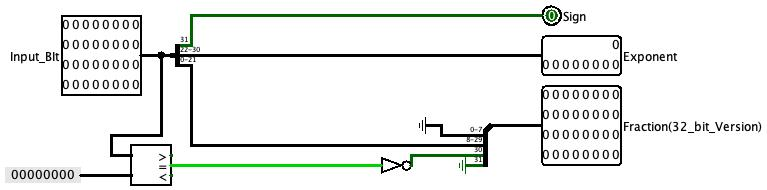
\includegraphics[width=0.8\textwidth]{Input_splitter.jpg} % Replace with actual image filename
\caption{Input Splitter module.}
\label{fig:input_splitter}
\end{figure}

\subsection*{LSE}
The LSE module processes inputs from two floating-point numbers, specifically:
\begin{itemize}
    \item Two 11-bit exponents.
    \item Two 1-bit sign values.
\end{itemize}
It outputs:
\begin{itemize}
    \item The fraction that needs to be shifted (associated with the smaller exponent).
    \item The fraction that does not need to be shifted.
    \item The difference between the two exponents (used to determine the shift amount).
\end{itemize}

\begin{figure}[h!]
\centering
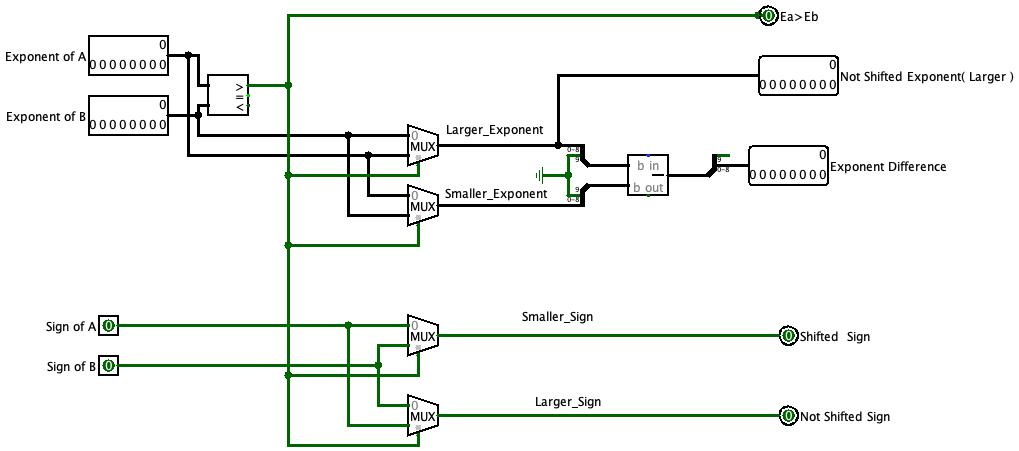
\includegraphics[width=0.8\textwidth]{LSE.jpg} % Replace with actual image filename
\caption{LSE module.}
\label{fig:lse_module}
\end{figure}

\subsection*{Updated Fraction}
This module takes two fractions as input:
\begin{itemize}
    \item The fraction to be shifted (corresponding to the smaller exponent).
    \item The fraction that remains unshifted (corresponding to the larger exponent).
\end{itemize}
It outputs:
\begin{itemize}
    \item The shifted fraction.
    \item The unshifted fraction.
\end{itemize}

\begin{figure}[h!]
\centering
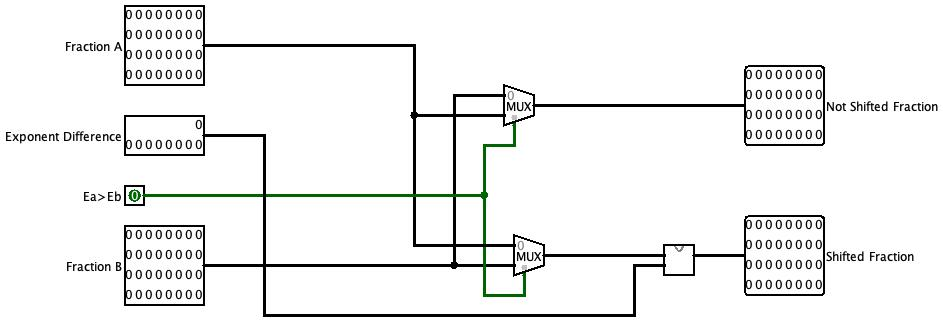
\includegraphics[width=0.8\textwidth]{Updated_fraction.jpg} % Replace with actual image filename
\caption{Updated Fraction module.}
\label{fig:updated_fraction}
\end{figure}
\subsection*{3.3 Shifter Library}
In floating point adders, shifters are essential for adjusting the fraction to normalize it or align it with the other operand. To implement this functionality, we used Logisim’s built-in splitters and multiplexers (muxes) to create two types of shifters: left and right shifters. The circuits in our shifter library include:

\begin{itemize}
    \item \textbf{Left Shifters:} 
    \begin{itemize}
        \item 1-bit left shifter (\texttt{1LeftShift})
        \item 2-bit left shifter (\texttt{2LeftShift})
        \item 4-bit left shifter (\texttt{4LeftShift})
        \item 8-bit left shifter (\texttt{8LeftShift})
        \item 16-bit left shifter (\texttt{16LeftShift})
    \end{itemize}
    
    \item \textbf{Right Shifters:} 
    \begin{itemize}
    \item 1-bit right shifter (\texttt{1\_bit\_right\_shift})
    \item 2-bit right shifter (\texttt{2\_bit\_right\_shift})
    \item 4-bit right shifter (\texttt{4\_bit\_right\_shift})
    \item 8-bit right shifter (\texttt{8\_bit\_right\_shift})
    \item 16-bit right shifter (\texttt{16\_bit\_right\_shift})
\end{itemize}


    \item \textbf{Arbitrary Shifters:} 
    These shifters can handle any bit shift operation from 1 to 31 bits.
    \begin{itemize}
        \item Arbitrary left shifter (\texttt{ArbLeftShift})
        \item Arbitrary right shifter (\texttt{Arbitary\_right\_shifter})
    \end{itemize}
    
    \item \textbf{Special Right Shifter:} 
    This right shifter ensures that any shifting greater than 31 bits results in all bits being set to 0.
    \begin{itemize}
        \item Right shifter with overflow handling (\texttt{right\_shift})
    \end{itemize}
\end{itemize}
\begin{figure}[h!]
\centering
\begin{minipage}{0.3\textwidth}
    \centering
    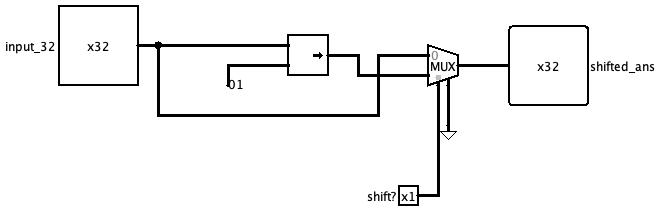
\includegraphics[width=\linewidth]{1bit.jpg}
    1 Bit Right Shifter
    \label{fig:1_bit_right_shift}
\end{minipage} 
\hfill
\begin{minipage}{0.3\textwidth}
    \centering
    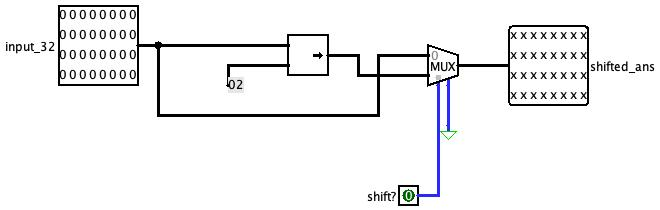
\includegraphics[width=\linewidth]{2.jpg}
    2 Bit Right Shifter
    \label{fig:2_bit_right_shift}
\end{minipage} 
\hfill
\begin{minipage}{0.3\textwidth}
    \centering
    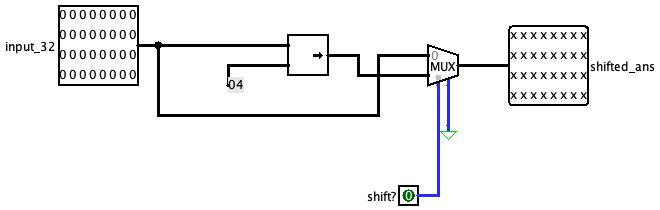
\includegraphics[width=\linewidth]{4.jpg}
    4 Bit Right Shifter
    \label{fig:4_bit_right_shift}
\end{minipage} 
\\
\vspace{0.5cm}
\begin{minipage}{0.3\textwidth}
    \centering
    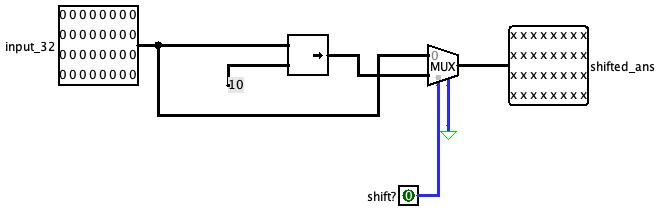
\includegraphics[width=\linewidth]{8.jpg}
    8 Bit Right Shifter
    \label{fig:8_bit_right_shift}
\end{minipage} 
\hfill
\begin{minipage}{0.3\textwidth}
    \centering
    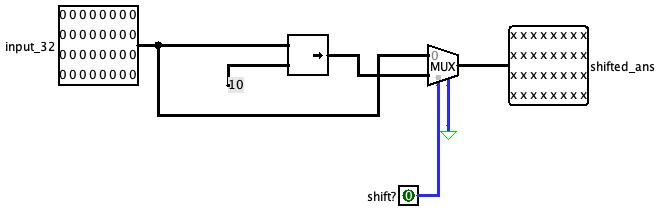
\includegraphics[width=\linewidth]{16.jpg}
    16 Bit Right Shifter
    \label{fig:16_bit_right_shift}
\end{minipage} 
\hfill
\begin{minipage}{0.3\textwidth}
    \centering
    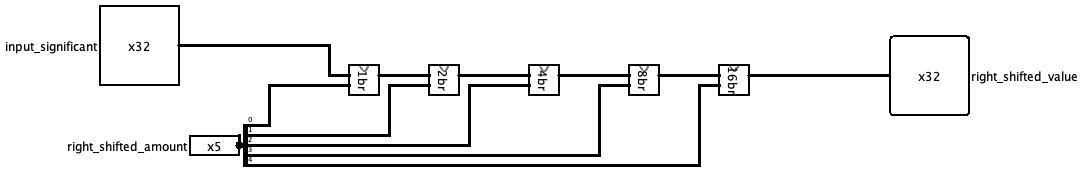
\includegraphics[width=\linewidth]{a.png}
    Arbitrary Right Shifter
    \label{fig:arbitrary_right_shift}
\end{minipage} 
\caption{Shifters used in the design}
\label{fig:shifters}
\end{figure}

% For the second image, the one with the right shift with empty
\begin{figure}[h!]
\centering
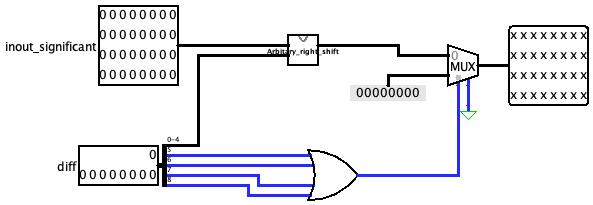
\includegraphics[width=0.6\textwidth]{r.jpg}  % Make the final image smaller
\caption{Right Shift With Empty}
\label{fig:right_shift_with_empty}
\end{figure}


\subsection*{3.5 Rounding Circuit}
The \texttt{Rounder.circ} module is designed to handle the rounding of the mantissa in the floating-point adder. It integrates two main components to achieve precise rounding:

\begin{itemize}
    \item \textbf{Comparator:} This component evaluates specific bits of the mantissa to determine whether rounding is necessary.
    \item \textbf{Full Adder:} Based on the comparator's result, the full adder adjusts the mantissa to perform the rounding operation.
\end{itemize}


\begin{figure}[h!]
\centering
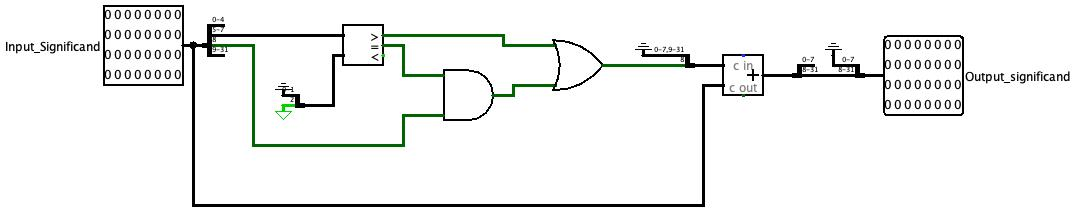
\includegraphics[width=0.8\textwidth]{Rounding.jpg} % Replace with actual image filename
\caption{Rounding Circuit module (\texttt{Rounder.circ}).}
\label{fig:rounding_circuit}
\end{figure}
\pagebreak
\subsection*{3.7 Third Party Libraries}
Third-party libraries \texttt{7400-lib.circ} and \texttt{logi7400dip.circ} are used to incorporate 7400 series ICs into the floating-point adder implementation. These libraries provide a modular and standardized approach for integrating logic gates and DIP IC models, ensuring efficient circuit design and compatibility.
\section*{5  High-level Block Diagram of the Architecture }
\begin{figure}[h!]
\centering
% Include your block diagram image here
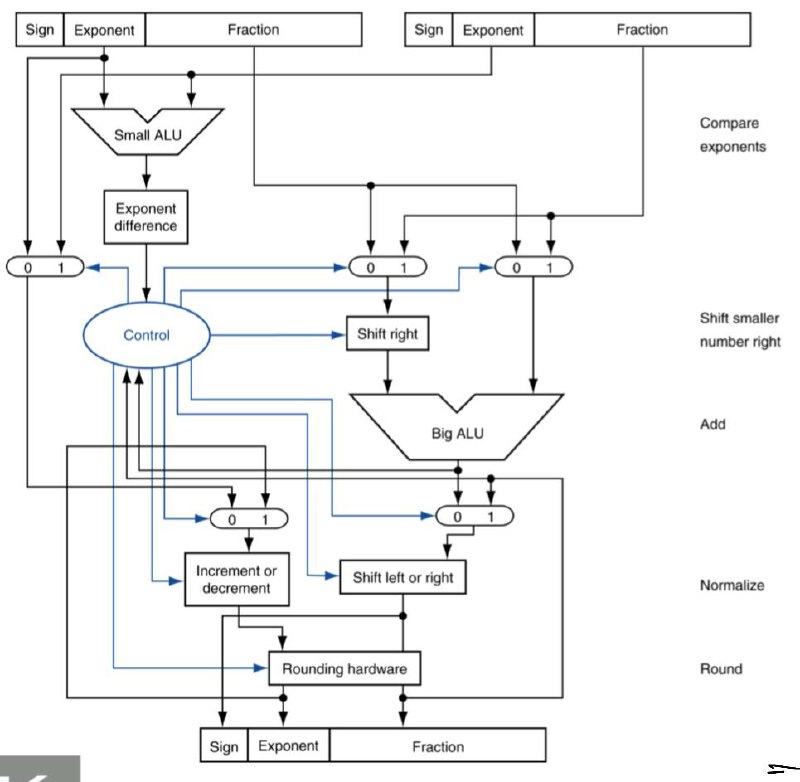
\includegraphics[width=\textwidth]{Block.jpg} 
\caption{Block Diagram of the Floating Point Adder (FPA)}
\label{fig:fpa_block_diagram}
\end{figure}
\section*{6. Comprehensive Design Description}
\subsection*{6.1 Comparing Exponents and Aligning the Radix Point}

To add two floating-point numbers, it is essential to align their radix points. This process ensures that both numbers are in the same scale before performing the addition. Typically, the alignment is achieved by shifting the number with the smaller exponent to the right. The difference between the exponents of the two numbers is calculated to determine the required number of shifts.

In our implementation, we utilized a subtractor to compute the difference between the two exponents, allowing for accurate alignment. The exponents are compared using a comparator to identify which input has the larger exponent. This ensures proper handling of the inputs and precise alignment of the radix points before proceeding to the addition stage.



\subsection*{6.2 Multiplexer-Based Shifting Mechanism}
The shifting process is implemented using a series of multiplexer-based shifters. Specifically, five 32-bit multiplexers are employed, each capable of performing shifts of 1, 2, 4, 8, or 16 bits. By combining these multiplexers, it is possible to achieve shifts of any length up to 31 bits. 

In cases where the required shift exceeds 31 bits, all bits of the smaller number are cleared to 0, effectively aligning it with the larger number. The input to the shifter circuit is derived from the exponent difference. To ensure accurate shifting, the lower five bits of the exponent difference are utilized while the upper seven bits are ignored. This design ensures that the maximum shift length does not exceed 31 bits (2\textsuperscript{5} - 1). If a larger shift is required, the fraction is cleared entirely, resulting in an output of zero.

\subsection*{6.3 Exponent Comparison and Radix Point Alignment}
To perform addition of two floating-point numbers, it is essential to align their radix points. This alignment is achieved by shifting the number with the smaller exponent to the right until it matches the larger exponent. The difference between the two exponents is calculated using a 9-bit subtractor, while a comparator determines which exponent is larger and the amount of shift required for proper alignment.
\subsection*{6.4 Rounding}
In our design, we use a 32-bit adder to perform the necessary additions and subtractions on the mantissas. However, since only 22 bits can be stored, sometimes rounding is required. The 23rd bit is reserved as the guard bit, and the 24nd bit is used for rounding. If any bits beyond the round bit are set, we activate the sticky bit. If no additional bits are set, the sticky bit remains inactive. We need to consider the following scenarios when performing rounding:

\begin{table}[h!]
\centering
\begin{tabular}{|c|c|c|c|c|}
\hline
\rowcolor{gray!20} \textbf{22nd bit} & \textbf{G} & \textbf{R} & \textbf{S} & \textbf{Action} \\ \hline
\rowcolor{white} X & 0 & X & X & Truncate \\ \hline
\rowcolor{gray!10} 1 & 1 & X & X & Round up \\ \hline
\rowcolor{white} 0 & 1 & 0 & 0 & Truncate \\ \hline
\rowcolor{gray!10} X & 1 & 1 & X & Round up \\ \hline
\rowcolor{gray!10} X & 1 & X & 1 & Round up \\ \hline
\end{tabular}
\caption{Rounding Behavior Based on Bits}
\end{table}
\noindent
\textbf{Note:} Truncation occurs only when the value of GRS is \( 100 \). Additionally, if the 22nd bit is 1, then 1 is added; otherwise, 0 is added.
K map for the whole process is give below :
\subsection*{6.5 Enhancing Precision}
In our design, we chose not to allocate a separate bit for capturing the overflow. Instead, we directly extracted this information from the carry-out. Additionally, we did not require a separate bit to indicate the sign during subtraction. Instead, the sign of the result was determined by examining the carry-out of the adder. If the carry-out is 1, the result is positive; if it's 0, the result is negative. Special handling is required when one of the summands is zero, which, as discussed in section 6.6, is dealt with separately. This approach effectively increases the precision by 2 bits.
\section*{7. ICs Used with Count}

The following table lists the ICs used in the design, along with their respective quantities:

\begin{table}[h!]
\centering
\begin{tabular}{|c|c|}
\hline
\textbf{IC} & \textbf{Quantity} \\ \hline
IC 7404 & 1 \\ \hline
IC 7408 & 5 \\ \hline
IC 7432 & 4 \\ \hline
IC 7486 & 1 \\ \hline
IC 74157 & 7 \\ \hline
\textbf{Total} & \textbf{18} \\ \hline
\end{tabular}
\caption{ICs Used with Quantity}
\end{table}

\noindent
The IC count is relatively low because we used Logisim's built-in libraries for adders , comparators and shifters , eliminating the need to design them from scratch or count their ICs.
Even above gate has not been used in IC gate formate rather Basic gate.
\section*{8. Simulator Used and Version}
The floating point adder circuit was simulated using Logisim version 2.7.1.

\end{document}
